\documentclass[pdf,9pt]{beamer}

%
% ADD PACKAGES here:
%
\usepackage{amsmath,amsfonts,graphicx}
\usepackage{braket}
\usepackage[skip=2ex plus1ex, indent=1ex]{parskip}

%\mode<presentation>{\usetheme{Warsaw}}
%\mode<presentation>{\usetheme{Copenhagen}}
%\mode<presentation>{\usetheme{Boadilla}}
\mode<presentation>{\usetheme{Madrid}}
%\useoutertheme{split}
\setbeamertemplate{footline}
{
  \leavevmode%
  \hbox{%
  \begin{beamercolorbox}[wd=.65\paperwidth,ht=2.25ex,dp=1ex,center]{author in head/foot}%
    \usebeamerfont{author in head/foot}\insertshortauthor
  \end{beamercolorbox}%
  \begin{beamercolorbox}[wd=.35\paperwidth,ht=2.25ex,dp=1ex,center]{title in head/foot}%
    \usebeamerfont{title in head/foot}\insertshorttitle\hspace*{3em}
    \insertframenumber{} / \inserttotalframenumber\hspace*{1ex}
  \end{beamercolorbox}}%
  \vskip0pt
}


\newcounter{lecnum}
\renewcommand{\thepage}{\thelecnum-\arabic{page}}
\renewcommand{\thesection}{\thelecnum.\arabic{section}}
\renewcommand{\theequation}{\thelecnum.\arabic{equation}}
\renewcommand{\thefigure}{\thelecnum.\arabic{figure}}
\renewcommand{\thetable}{\thelecnum.\arabic{table}}


\renewcommand{\cite}[1]{[#1]}
\def\beginrefs{\begin{list}
        {[\arabic{equation}]}{\usecounter{equation}
         \setlength{\leftmargin}{2.0truecm}\setlength{\labelsep}{0.4truecm}%
         \setlength{\labelwidth}{1.6truecm}}}
\def\endrefs{\end{list}}
\def\bibentry#1{\item[\hbox{[#1]}]}



%%
\title[PH 421 Project Presentation]{Quantum Non-linear Optics with Single Atoms and Virtual Photons}
% \subtitle{The f*ck are we doing?}

\author[Group 1]{Group 1 \\
Bhavana Parankusam, Kaustav Prasad, Namita Agrawal,\\
Rehmat Singh Chawla, Samyak Jain}
\institute{Physics Department - IIT Bombay}
\date{}

\begin{document}
    \begin{frame}
      \titlepage
    \end{frame}
    \begin{frame}{Introduction}
        A number of non-linear effects can be realised with one or more atoms coupled to one or more resonator modes. To achieve this, we need to construct an interaction between an electromagnetic mode and a two-level atom, which is given by the quantum Rabi Hamiltonian.
        
       We require a very strong light-matter coupling for the non-linear effects to be noticeable.
       
       In this model, we use excitations of resonators modes as opposed to propagating waves used conventionally. We do not require any external drive, and realise the non-linear effects with a minimum number of photons.
         
        
    \end{frame}
    \begin{frame}{Hamiltonian for Light Matter Interaction}
    Considering only the electric dipole interaction, we can derive via the Quantisation of the Electric Field the Hamiltonian for the interactions of 2-level atoms and photons. The General Quantum Rabi Hamiltonian is: \\
    
$$
\hat{H}_{gen}^{Rabi} =  \Sigma_k \omega_k \hat{a}_k^\dagger \hat{a}_k + \frac{1}{2} \omega_q \hat{\sigma}_z + \Sigma_kg(\hat{a}_k + \hat{a}_k^\dagger)(\hat{\sigma}_x \cos{\theta} + \hat{\sigma}_z\sin{\theta})
$$
    With only longitudinal coupling this simplifies to:
$$
\hat{H}^{Rabi} = \Sigma_k\omega _k \hat{a}^\dagger_k \hat{a}_k + \frac{1}{2}\omega_q \hat{\sigma}_z + \Sigma_k g(\hat{a}_k + \hat{a}_k^\dagger)(\hat{\sigma}_- + \hat{\sigma}_+)
$$

Further, when the transition frequency of the atom is close to the frequency of the photons, using the rotating wave approximation this simplifies to:
$$
\hat{H}^{JC} = \omega _a \hat{a}^\dagger \hat{a} + \frac{1}{2}\omega_q \hat{\sigma}_z + g(\hat a \hat{\sigma}_+ + \hat{a}^\dagger\hat{\sigma}_-)
$$
which is called as the Jaynes-Cumming Model. In all these Hamiltonians, we are working in a tensor product of the Fock State Basis of Photons and a phase space of the 2-level atom isomorphic to that of a spin-half particle. Now we discuss how we can use such a system to show various well-known optical phenomena.
    \end{frame}

    \begin{frame}{The Effective Interaction Hamiltonian}
    We decompose $\hat H_\text{int}$ into $g_\text{eff}(i,f) |f\rangle \langle i|$ type terms, with the end goal being to maximise a particular $g_\text{eff}(i,f)$ and write $\hat H_\text{int}^\text{eff} = g_\text{eff}(i,f) |f\rangle \langle i| + g^*_\text{eff}(i,f) |i\rangle \langle f|$.

Assuming an $n$-step path is the lowest-order path which can take $|i\rangle$ to $|f\rangle$, to lowest order $g_\text{eff}$ is:
$$
g_\text{eff} = \sum_{j_1,\dots,j_{n-1}}\frac{V_{fj_{n-1}}\dots V_{j_1i}}{(E_i-E_{j_{n-1}})\dots(E_{i}-E_{j_1})}^\S
$$

Up to a phase factor. Here, $V_{ij} := \langle i|\hat H_{int}|j\rangle$.


The summation over ${j_1,\dots,j_{n-1}}$ can be intuitively understood as a summation over various paths that can take $|i\rangle$ to $|f\rangle$. A path is a valid one if all pairs of consecutive states in the path $|j_{\mu-1}\rangle,|j_\mu\rangle$ are connected by the interaction hamiltonian - all $V_{j_\mu j_{\mu-1}}$ must be non-zero.

\hfill\newline
$^\S$We derive this expression in Appendix A of the report using perturbation theory.
    \end{frame}

\begin{frame}{Calculation of $g_\text{eff}$}
Take the following path, one of the many contributing to a down-conversion process
$$
|1,0,g\rangle\xrightarrow{\hat b^\dagger\hat\sigma_z}|1,1,g\rangle\xrightarrow{\hat a \hat\sigma_+}|0,1,e\rangle\xrightarrow{\hat b^\dagger\hat\sigma_+}|0,2,g\rangle
$$

Name $i=|1,0,g\rangle, n = |1,1,g\rangle, m=|0,1,e\rangle, f = |0,2,g\rangle $

Then the component of $g_\text{eff}$ is
$$
\frac{V_{fm}V_{mn}V_{ni}}{(E_m-E_i)(E_n-E_i)}
$$%\vspace*{-4ex}
Using the generalised Rabi hamiltonian with $\hat H_0 = \omega_a \hat a^\dagger\hat a+\omega_b\hat b^\dagger\hat b + \frac 1 2 \omega_q\hat\sigma_z$
and $\hat H_{int} = (g_a(\hat a+\hat a^\dagger)+g_b(\hat b+\hat b^\dagger))(\hat\sigma_z\sin\theta+(\hat\sigma_++\hat\sigma_-)\cos\theta))$,
\begin{align*}
V_{fm} = \langle f|\hat H_{int}| m\rangle = \sqrt{2}g_b\cos\theta, 
V_{mn} &= \langle m|\hat H_{int}| n\rangle = g_a\cos\theta, 
V_{ni} = \langle n|\hat H_{int}| i\rangle = g_a\sin\theta
\\
E_m =  \langle m|\hat H_{0}| m\rangle = \frac 1 2\omega_q+\omega_b, 
E_n &= \omega_a + \omega_b - \frac 1 2 \omega_q,
E_i = \omega_a - \frac 1 2 \omega_q
\\[0.5ex]
\therefore g_\text{eff}^\text{chosen path} &= \frac{\sqrt{2}g_a g_b^2 \cos^2\theta\sin\theta}{(\omega_q+\omega_b-\omega_a)\omega_b}
\end{align*}
    
\end{frame}

    
    \begin{frame}{Three Wave Mixing}
    \begin{itemize}
        \item SFG and DFG are the most general forms of three wave mixing.
        
                In quantum NL optics, SFG can be described as: 
        
        $$\ket{n_1, n_2, n_+} \rightarrow \ket{n_1 - 1, n_2 - 1, n_+ + 1}$$
    
    \item Multiple resonator-qubit setups are possible that can serve as analogs to three wave mixing. For example, if we couple three resonators and one qubit, then the transition  $\ket{1,1,0,g} \rightarrow \ket{0,0,1,g}$  corresponds to SFG, while the transition in reverse corresponds to DFG.
    
    \item Through light-matter coupling, we obtain an additional degree of freedom to make the lower order processes be off-resonance; thus the lower order processes do not limit the efficiency of higher order processes.

    \end{itemize}
    
    For example, when the resonance condition for SFG i.e. $\omega_1 + \omega_2 \approx \omega_+$ is met, we can ensure that the intermediate state $|{1,0,0,e}\rangle$ with the energy $\omega_1 + \omega_q$ (which is reachable via a lower order process) will be far off resonance if we choose $\omega_q$ sufficiently far from $\omega_2$.

    \end{frame}
    
    \begin{frame}{}
         \begin{center}
            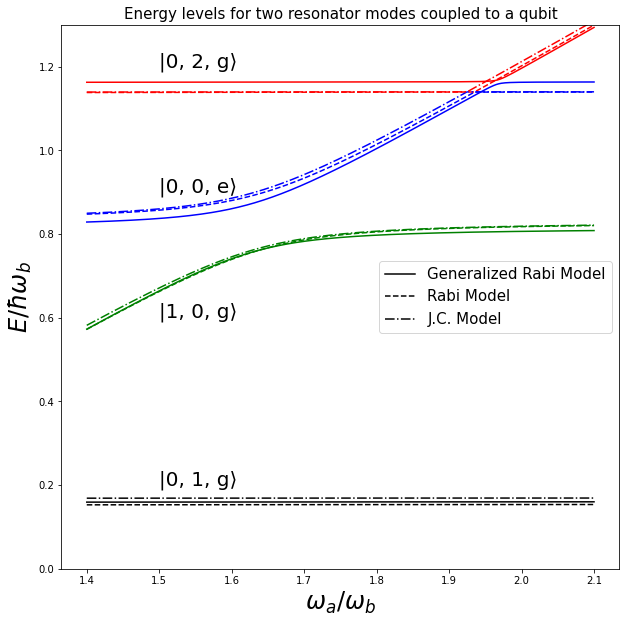
\includegraphics[scale=0.4]{fig3_paper_plot.png}
        \end{center}
    \end{frame}

    \begin{frame}{Experimental Feasibility}
        For the interaction to be observable, the parameter we need to consider is the coupling strength for the interaction between qubit and photon mode. It needs to be greater than the dissipation rates of the atom and photon. i.e. $$g> \kappa, \gamma$$
        
        Where $\kappa$  is the resonator loss, $\gamma$ is the qubit decoherence rate.
        For it to have close to unit efficiency, the Ultra Strong coupling regime is preferred. i.e. $$g\gg \omega_{1}, \omega_{+}$$
        
        Circuit Quantum Electrodynamics is a good candidate to implement the theory we have described. Superconducting circuits with Josephson junctions can act as artificial atoms and placing them in a  cavity enhances the coherent oscillations.
        
        $\omega_{1}, \omega_{q} \approx GHz, \gamma $ of the order kHz and Quality factor ($\omega/\kappa$) of the order $10^{6}$ has been achieved. 
        
    \end{frame}
\end{document}
